\begin{figure}[ht]
    \centering
    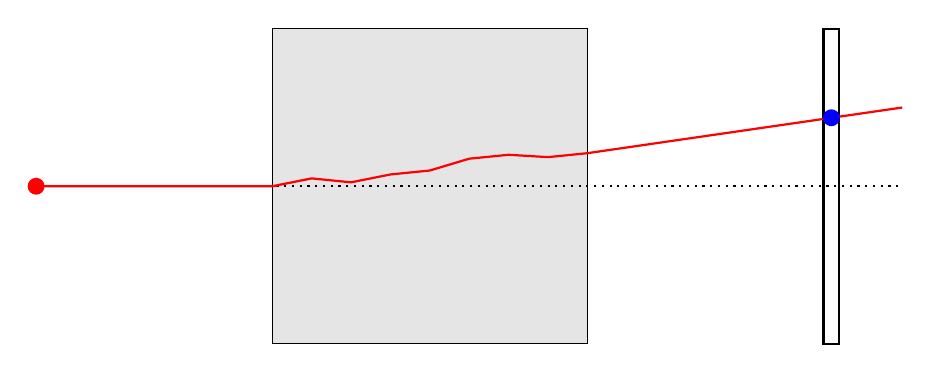
\begin{tikzpicture}
        \filldraw[red] (-5,0) circle (0.1);
        \draw[fill=gray!20] (-2,-2) rectangle (2,2);
        \draw[black, thick] (5,-2) rectangle (5.2,2);

        \draw[black, thick, dotted] (-5,0) -- (6,0);
        \draw[red, thick] (-5,0) -- (-2,0) -- (-1.5,0.1) -- (-1,0.05) -- (-0.5,0.15) -- (0,0.2) -- (0.5,0.35) -- (1,0.4) -- (1.5,0.37) -- (2,0.42) -- (6,1);
        \filldraw[blue] (5.1,0.87) circle (0.1);
    \end{tikzpicture}
    \caption{Illustration of the toy model. The box represents the dense material. The screen is placed at some distance to the box. Muons are emitted from a source on the left side of the box and their hits are recorded on the screen indicated with a blue dot.}
    \label{fig:dev/dense/toy-model}
\end{figure}
